
\section{Simulation num\'erique}

\subsection{Syst\`eme \'etudi\'e}
Pendant les simulations num\'eriques au cas g\'en\'erique on est capable 
d'\'etudier le syst\`eme de $N$ satellites (d\'ebris) observ\'es par $M$
t\'elescopes. Pour cela on utilise les solutions connues des \'equations 
de mouvement: 
% \begin{center}
% 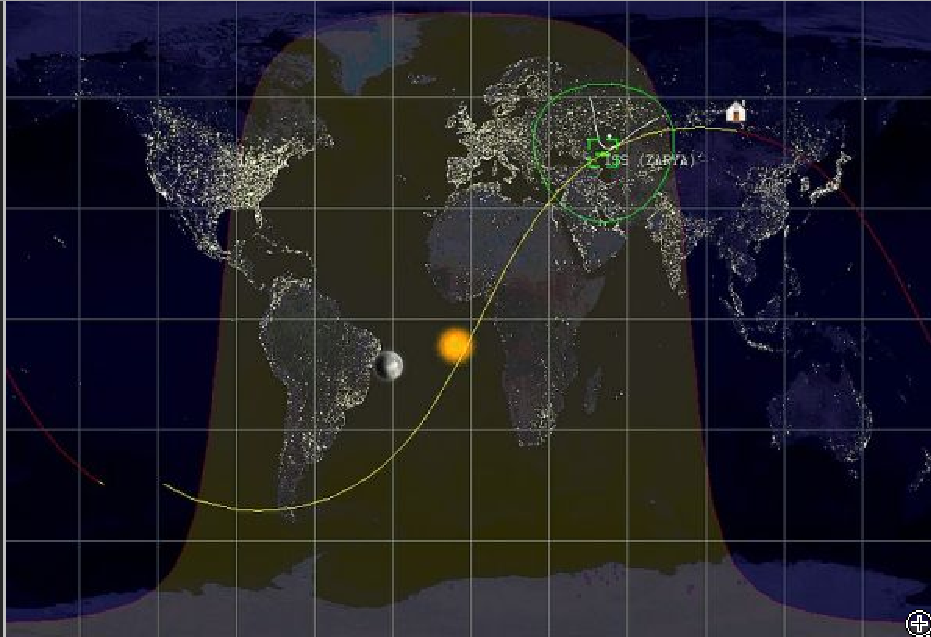
\includegraphics[width = 0.75\linewidth]{map2.pdf} 
% \end{center}
\begin{align}
   \theta_{O_i}(t) &= \theta_{O_i}(t_0) + (t-t_0)\dot \theta_{O_i} &  \nonumber \\
   \theta_{D_i}(t) &= \theta_{D_i}(t_0) + (t-t_0)\dot \theta_{D_i}  & i = 1, \dots N \label{vladimir:sat} \\
   \theta_{T_j}(t) &= \theta_{T_j}(t_0) + (t-t_0)\dot \theta_{T_j} & j = 1, \dots M \label{vladimir:tel} \\
   \theta_S(t) &= \theta_S(t_0) +  (t-t_0)\dot\theta_S  &\label{vladimir:sun} 
\end{align}
Ici les deux premi\`eres \'equations sur $\theta_{O_i}$ et
$\theta_{D_i}$ caract\'erisent la position du $i$'\`eme satellite par
rapport \`a un rep\`ere fixe; la troisi\`eme \'equation sur
$\theta_{T_j}$ est expliqu\'ee par la rotation de la Terre et
caract\'erise donc la position des t\'elescopes; la derni\`ere
\'equation d\'efinit l'évolution de la direction du Soleil.

La trajectoire typique du satellite (dans un rep\`ere fixe) va « colorer » une partie de
la sph\`ere de rayon correspondant \`a l'altitude de satellite, ou plus pr\'ecis\'ement la sph\`ere
sans les « chapeaux » autour des p\^oles, donn\'es par l'angle d'inclinaison d'orbite
(voir \autoref{vladimir:repfx})
 \begin{figure}[htp] \centering
     \includegraphics*[width=3in, height=3in]{repfx.png}
      \caption{
            \label{vladimir:repfx}
Trajectoire de satellite dans un syst\`eme des coordonn\'ees fixe. }
 \end{figure}

 %% Note de Antoine : la figure est incompréhensible sans les axes, je
 %% la commente ...


 
% Sa projection sur la Terre tournante est donn\'ee sur la \autoref{vladimir:mks}. 
% On a l'habitude de voir les trajectoires comme celle-ci dans les
% centres de contr\^ole des missions spatiales.
%  Comme on le voit clairement, la trajectoire g\'en\'erique n'est pas p\'eriodique
%  (\autoref{vladimir:mks}, zone entourée).


% \begin{figure}[htp] \centering
%       \includegraphics*[height=3in]{mks.png}
%       \caption{
%             \label{vladimir:mks}
% Proj\'ection de traj\'ectoire de satellite}
%  \end{figure}
 

\subsection{La loi de probabilit\'e d'observation}
La premi\`ere s\'erie des tests num\'eriques a pour but de v\'erifier
l'hypoth\`ese de la loi de probabilit\'e d'observer un satellite 
donn\'e avec un t\'elescopes donn\'e. 
Comme \`a chaque instant on connait la position du satellite et du t\'elescope
(équations (\ref{vladimir:sat}, \ref{vladimir:tel})), on peut comparer ses coordonn\'ees sph\'eriques 
et conclure si le satellite est dans le champ de vue de t\'elescope.

% Sur la \autoref{vladimir:mks} cette situation correspond \`a l'intersection de la projection de la
% trajectoire avec la zone bleue, repr\'esentant le t\'elescope.
% (L'image est bien sûr sch\'ematique: pour la vraie taille du champ de vue de t\'elescope
% utilis\'ee dans les simulation, voir la section sur l'observabilit\'e d'une orbite.)

Le test num\'erique est donc une simulation de mouvement de $N$ satellites
tous sur l'orbite avec le m\^eme angle d'inclinaison $i_d$ de la valeur proche (mais pas \'egale) 
\`a la valeur correspondante aux satellites h\'eliosynchrones, mais avec une l\'eg\`ere diff\'erence 
al\'eatoire de vitesse angulaire et la phase sur l'orbite. Pour le moment on 
ne prend pas en compte les conditions d'\'eclairage. 

La d\'ependance de nombre des satellites rep\'er\'es de temps d'observation
est donn\'ee sur la \autoref{vladimir:stat}. 
 \begin{figure}[htp] \centering
      \includegraphics*[height=3in]{stat.png}
      \caption{
            \label{vladimir:stat}
  Proportion des satellites rep\'er\'es pour  $N = 100$ en vert, $N = 1000$ en bleu, $N = 5000$ en rouge, courbe th\'eorique
  en noir}
 \end{figure}
Qualitativement elle correspond bien \`a notre estimation th\'eorique m\^eme avec la loi
binomiale.  

Ce r\'esultat montre entre autres que l'hypoth\`ese de l'ind\'ependance 
d'observer le satellite pendant deux jours cons\'ecutifs est 
bien valable au d\'ebut d'observation. 
% La diff\'erence quantitative entre la probabilit\'e estim\'ee est simul\'ee
% est de 0,XX\%.  %L\`a je ne souviens plus...

Pour des temps plus longs, le comportement est plus subtil, comme on
peut le voir en échelle logarithmique (\autoref{vladimir:stat_log})

\begin{figure}[ht] \centering
      \includegraphics*[height=3in]{stat_log.png}
      \caption{
            \label{vladimir:stat_log}
  Proportion des satellites non-rep\'er\'es \`a l'\'echelle logarithmique $N = 100$ en vert, $N = 1000$ en bleu, $N = 5000$ en rouge, estimation th\'eorique
  de la loi binomiale en noir}
 \end{figure}

Un modèle plus avancé, prenant en compte les défauts d'ergodicité,
doit donc être utilisé. Pour le vérifier, il faudrait des simulations
plus longues et précises, que nous n'avons pas eu le temps de faire.  
\subsection{Condition d'\'eclairage et ergodicit\'e}  
Pour la deuxi\`eme s\'erie des simulations on ajoute la condition d'\'eclairage, c'est-\`a-dire 
si le d\'ebris est dans le champ de vue de t\'elescope il est consid\'er\'e comme rep\'er\'e
si le d\'ebris est \'eclair\'e et le t\'elescope ne l'est pas. Cela est g\'er\'e par la prise 
en compte de position du Soleil (\autoref{vladimir:sun}) --- voir la section 
« Conditions d'\'eclairement » pour les d\'etails. 

Le but de cette s\'erie des tests num\'eriques est \`a la fois de v\'erifier 
l'ind\'ependance (moyenne) de condition de visibilit\'e g\'eom\'etrique (position
relative de satellite et de t\'elescope) et d'\'eclairage (position
du Soleil) ainsi que d'\'etudier l'effet d'augmentation de nombre des
t\'elescopes. 

% {\small Calcul: cluster de l'ICJ Univ. Claude Bernard Lyon 1}
Le tableau suivant montre le nombre des d\'ebris observ\'es
\`a la fin de la simulation pour les diff\'erents temps d'observation et nombres des
t\'elescopes. Ici on fait varier tous les param\`etres du syst\`eme.

\begin{center}
\begin{tabular}{|c|c|c|c|} \hline
 D\'ebris & T\'el\'escopes & Temps & \% vus \\ 
 \hline \hline
 100 & 10 & $\sim$ 2 mois &82 \\
 \hline
 100 & 2 & $\sim$ 10 mois &89 \\
 \hline
 \hline
 1000 & 10 & $\sim$ 2 mois &85.5 \\
 \hline
 1000 & 5 & $\sim$ 4 mois &86.7 \\
 \hline
 1000 & 2 & $\sim$ 10 mois &87.7 \\
 \hline  
 \hline
 10000 & 10 & $\sim$ 2 mois &84.0 \\
 \hline
 \hline
 $10^5$ & 14 & $\sim$ 8 mois &  94.7 \\
 \hline
\end{tabular} 
\end{center}
  % {\small Calcul: cluster de l'ICJ Univ. Claude Bernard Lyon 1}
Ceci est coh\'erent avec la probabilit\'e journali\`ere d'observation 
   $p \approx 1\%$, ce qui est bien la valeur estim\'ee suivant l'hypoth\`ese 
   d'ind\'ependance pour les simulations courtes. 
   
   De plus on voit que la probabilit\'e d'observation \`a la fin de p\'eriode
   est la m\^eme quand le produit de temps d'observation et le nombre des t\'elescopes
   coïncide. On observe donc « le premier pas vers l'ergodicit\'e », quand la moyenne 
   temporelle est \'egale \`a la moyenne de l'ensemble. 
   
   \subsection{Impl\'ementation}
On va conclure la section de simulation par quelques mots sur l'impl\'ementation.
Tout d'abord l'algorithme utilis\'e est assez direct comme on \'etudie les solutions 
connues des \'equations de mouvement (\ref{vladimir:sat}, \ref{vladimir:tel}, \ref{vladimir:sun}). On a analys\'e la trajectoire enti\`ere de chaque d\'ebris m\^eme si cela n'est pas vraiment 
n\'ecessaire pour la statistique d'observation des d\'ebris.

On peut proposer plusieurs pistes de l'am\'elioration de la m\'ethode. 
%(non-impl\'ement\'ees, faute de temps).
La simulation utilis\'ee est assez simpliste au sens qu'on mod\'elise le ph\'enom\`ene m\^eme quand il
 ne nous int\'eresse pas, c'est-\`a-dire on \'etudie les parties longues des orbites pour lesquelles on est sûr 
qu'elle n'intersectent pas le champ de vue du t\'elescope. Pour \'eviter cela on peut estimer le temps de prochaine
intersection de l'orbite du d\'ebris avec la trajectoire du t\'elescope et \'etudier cette p\'eriode avec plus de pr\'ecision. 
C'est direct pour un seul t\'elescope et assez facile pour plusieurs. On remarque \'egalement que les simulations
pour les trajectoires des d\'ebris distincts sont ind\'ependantes,
c'est-\`a-dire que l'algorithme de calcul d'estimation de la
probabilit\'e d'observation est parall\'elisable avec un gain lin\'eaire. 
   
   
